\documentclass[11pt, twocolumn]{article}
\usepackage[margin=0.25in]{geometry}
\usepackage{amsmath}
\usepackage{graphicx}
\graphicspath{{images/}}
\title{AM1 Reparameterization Using a Genetic Algorithm}
\author{Dustin Tracy}
\begin{document}
\maketitle
\begin{abstract}
\textbf{We apply a hybrid genetic algorithm to the AM1 parameter set in order to find a set of paremeters that beter matches the outputs produced by B3LYP\@.
Forces, excited state energies, and the ground energies among multiple geometries are used to deterime fitness.}
\end{abstract}
\section{Introduction}
In computational chemistry it is often unfeasable to do a full quantum mechanical calculation of molecular mechanics.
Certain approximations must be made.
Many of these approximations fall under the classification of semi-empiracle methods, including AM1, PM6, MNDO and a few others.
The parameters of these methods are choosen to be effective for a very broad range of molecules.
In this paper, our focus is on the AM1(Austin Model 1) method developed in 1985.
In 2006, a new method, RM1, was created based of a reparameterization of AM1 to better fit with the most common biological atoms.
However, RM1 kept the AM1 methodology and only changed the parameters.
In this paper we attempt to reparameterize AM1 to beter match the outputs B3LYP for a specific class of molecules using hybrid genetic algorithm.
\section{Methodology}
\subsection{The Modified Genetic Algorithm}
The genetic algorithm tries to simulate natural evolution for the optimization of AM1 parameters.
Though an elite class modification is made to help with convergence.
Each of the AM1 parameters are treated as a gene. 
The parameters EHEAT and EISol are kept constant.
The set of parameters is treated as an individual.
Many individuals are created using random perturbations of a host set to fill a population.
The fitness of each individual is measured.
The worst indiviuals are eliminated.
The best from the remaining individuals are placed into an elite class, while the others are placed into a peasant class.
Single slightly mutated copies of the elites are created.
The mutated copies are compared to their progenerators, and the least fit are eliminated.
The survivors of this elimination form the new elites.
The elites and the peasants then take part in a breeding precedure.
The breeding precedure consists of randomly pairing any two survivors and creating a new mixed copy.
The most fit individuals are more likely to be paired, however, fitness is not taking into account during the mixing precedure.
Each parent individual will contribute around half of their genome to the child individual.
The peasants are then eliminated and only the elites and the child individuals form a new population.
The fitness of each individual is measures and the cycle continues for predetermined number of generations.
\subsection{Fitness Function}
The optimized minimization geometry using B3LYP is used as base geometry.
Each atom from this base geometry is uniformly perturbed to create $G$ new geometries.
These geometries remain constant throughout the algorithm.
Fitness is then determined through a function of three other fitness measures: Force Fitness, Ground State Fitness, and Excited State Fitness.

Force fitness for each geometry is
\begin{equation*}
  \mathcal{F}_{force}^{g}=\displaystyle\sum_{i=1}^{N}\frac{(\hat{\mathbf{F}}_{AM1}^{i}\cdot\hat{\mathbf{F}}_{DFT}^{i}-1)}{N}
\end{equation*}
where $\hat{\mathbf{F}}$ are the force vectors for each atom and $N$ is the number of atoms.
Overall force fitness is the average of these values.

Excited state fitness for each geometry is
\begin{equation*}
  \mathcal{F}_{ES}^{g}=\displaystyle\sum_{i=1}^{N}\frac{{\left(E_{AM1}^{i}-E_{DFT}^{i}\right)}^{2}}{N}
\end{equation*}
where $N$ is the number of excited states and $E$ the enery of each excited state.
The average over the geometries is the overall excited state fitness.

Ground state energy fitness is
\begin{equation*}
  \mathcal{F}_{ground}=\displaystyle\sum_{i=1}^{G}{\left(E_{AM1}-E_{DFT}\right)}^{2}
\end{equation*}
where $E$ is the ground state energy. No additional calculations are needed for the overall ground state fitness.

Total fitness is given by
\begin{equation*}
  \mathcal{F}={\left(\alpha\frac{\mathcal{F}_{force}}{\mathcal{F}_{force}^{i}} +
              \beta\frac{\mathcal{F}_{ES}}{\mathcal{F}_{ES}^{i}} +
              \gamma\frac{\mathcal{F}_{ground}}{\mathcal{F}_{ground}^{i}}\right)}
              /{\left(\alpha + \beta + \gamma\right)}
\end{equation*}
where the fitness of the initial AM1 parameters is given by $Fi$.
$\alpha$, $\beta$, and $\gamma$ are the weights of each fitness.
These weights were determined empirically by running the algorithm a numerous times while keeping record of how much each decreased.
The fitness that decreased the most was given a smaller weight, forcing the algorithm to distribute the optimization.
Techniques to automate this determination of $\alpha$, $\beta$, and $\gamma$ exist and will be included in the future implementations.

\section{Results}
\begin{figure}[total]
  \centering
  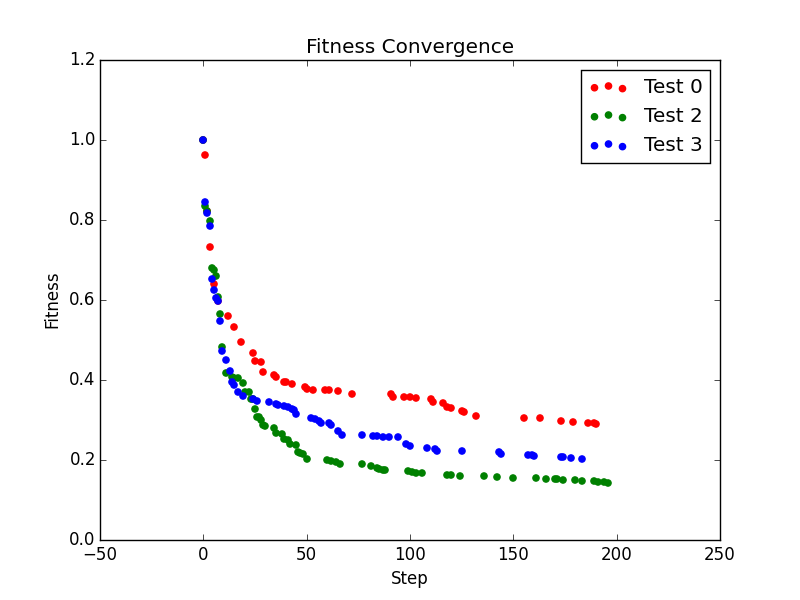
\includegraphics[width=0.5\textwidth]{furan_convergence}
  \caption{Total fitness convergence for three runs of the genetic algorithm on Furan for 200 generations.
  24 population was used with 2 elites with 10\% perturbation and mutation rate and 50\% survival}
\end{figure}

\begin{figure}[force]
  \centering
  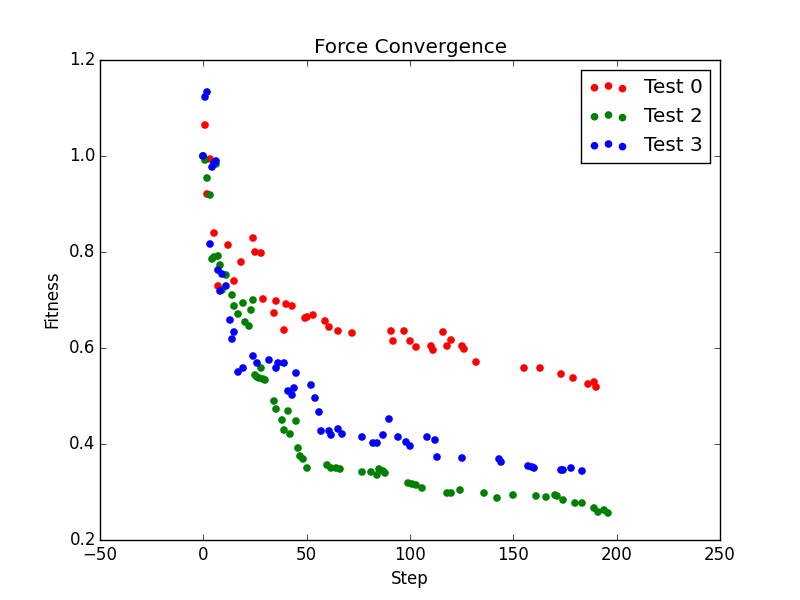
\includegraphics[width=0.5\textwidth]{furan_force_convergence}
  \caption{Force fitness convergence for three runs of the genetic algorithm on Furan for 200 generations.
  24 population was used with 2 elites with 10\% perturbation and mutation rate and 50\% survival}
\end{figure}

\begin{figure}[es]
  \centering
  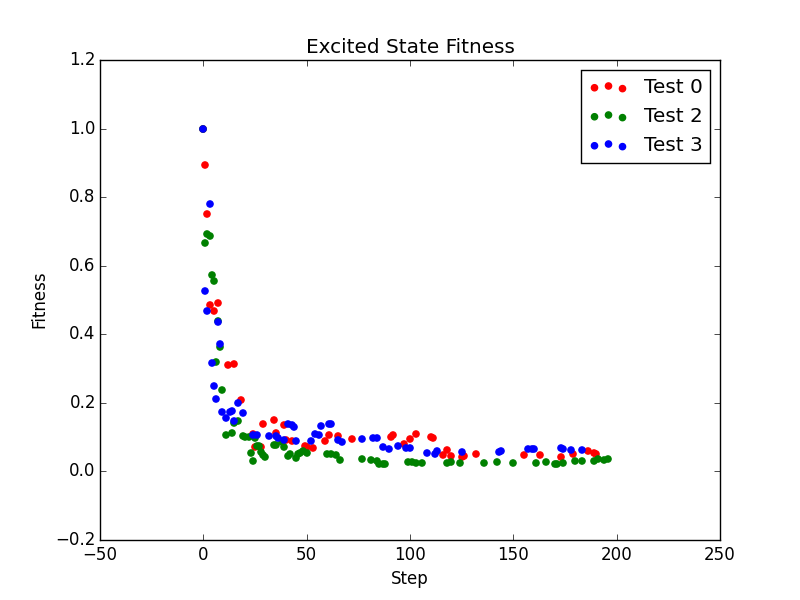
\includegraphics[width=0.5\textwidth]{furan_es_convergence}
  \caption{Excited state fitness convergence for three runs of the genetic algorithm on Furan for 200 generations.
  24 population was used with 2 elites with 10\% perturbation and mutation rate and 50\% survival}
\end{figure}

\begin{figure}[ground]
  \centering
  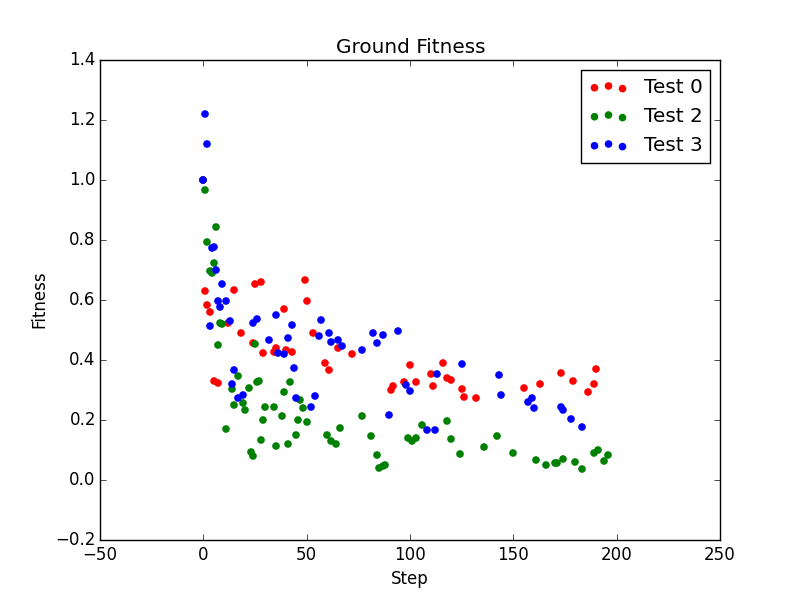
\includegraphics[width=0.5\textwidth]{furan_ground_convergence}
  \caption{Ground energy fitness convergence for three runs of the genetic algorithm on Furan for 200 generations.
  24 population was used with 2 elites with 10\% perturbation and mutation rate and 50\% survival}
\end{figure}

\begin{figure}[IR0]
  \centering
  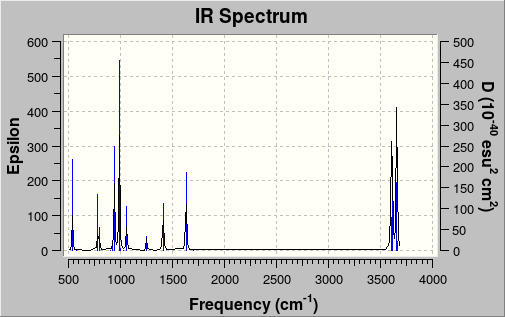
\includegraphics[width=0.5\textwidth]{IR_0}
  \caption{IR Spectrum for Furan test 0}
\end{figure}

\begin{figure}[IR1]
  \centering
  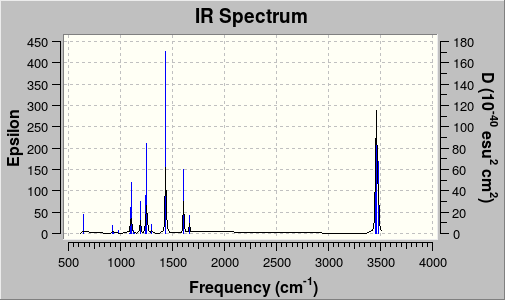
\includegraphics[width=0.5\textwidth]{IR_1}
  \caption{IR Spectrum for Furan test 1}
\end{figure}

\begin{figure}[IR2]
  \centering
  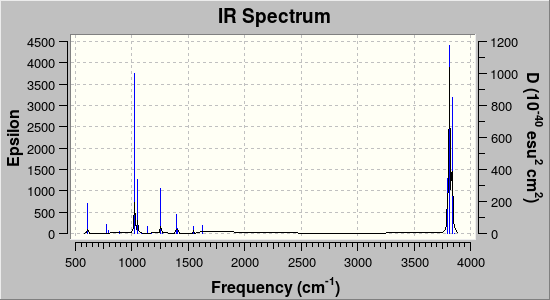
\includegraphics[width=0.5\textwidth]{IR_2}
  \caption{IR Spectrum for Furan test 2}
\end{figure}

\begin{figure}[IR_DFT]
  \centering
  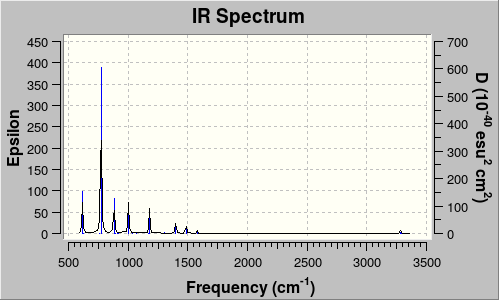
\includegraphics[width=0.5\textwidth]{IR_DFT}
  \caption{IR Spectrum for Furan at the DFT level}
\end{figure}


\end{document}
